\section{Resultados}

Neste capítulo serão apresentados os resultados encontrados com as entrevistas baseadas no processo de análise de dados apresentada no capítulo anterior. Primeiramente será abordado como foi feito o agrupamento dos códigos gerados com as práticas. Após isso, será focado o estudo do predomínio das práticas em Recife, seguido da análise de coerência do \emph{Stairway to Heaven}. Por fim, serão apresentados princípios e práticas subjacentes que governam a adoção de CI/CD na amostra.


\subsection{Estudo de Predomínio das Práticas}

Com o intuito de responder a pergunta de pesquisa RQ1 -- \emph{Quais as práticas de CI/CD são utilizadas pelas empresas em Recife?} -- de forma restrita aos 11 entrevistados das 7 empresas da amostra, foi montada a Tabela \ref{tabela_t3}, demonstrando a utilização de cada uma das práticas definidas para cada um dos participantes. Nesta, é demonstrada através da coloração da célula o grau de utilização de determinada prática por determinado participante. Assim, o verde mais escuro significa que o participante utiliza totalmente, enquanto o verde claro significa utilização parcial e, por fim, o branco denota a não utilização. Esta foi produzida a partir da Tabela Entrevistado-Pratica-Codigos, retirando-se os códigos agrupados e ordenando as colunas pela utilização de determinada prática. A ideia é replicar a Tabela 1 do artigo base \cite{empiricalStudy2016}, presente na Figura \ref{tabela_1_artigo_base}.

\begin{table}[ht]
\begin{center}
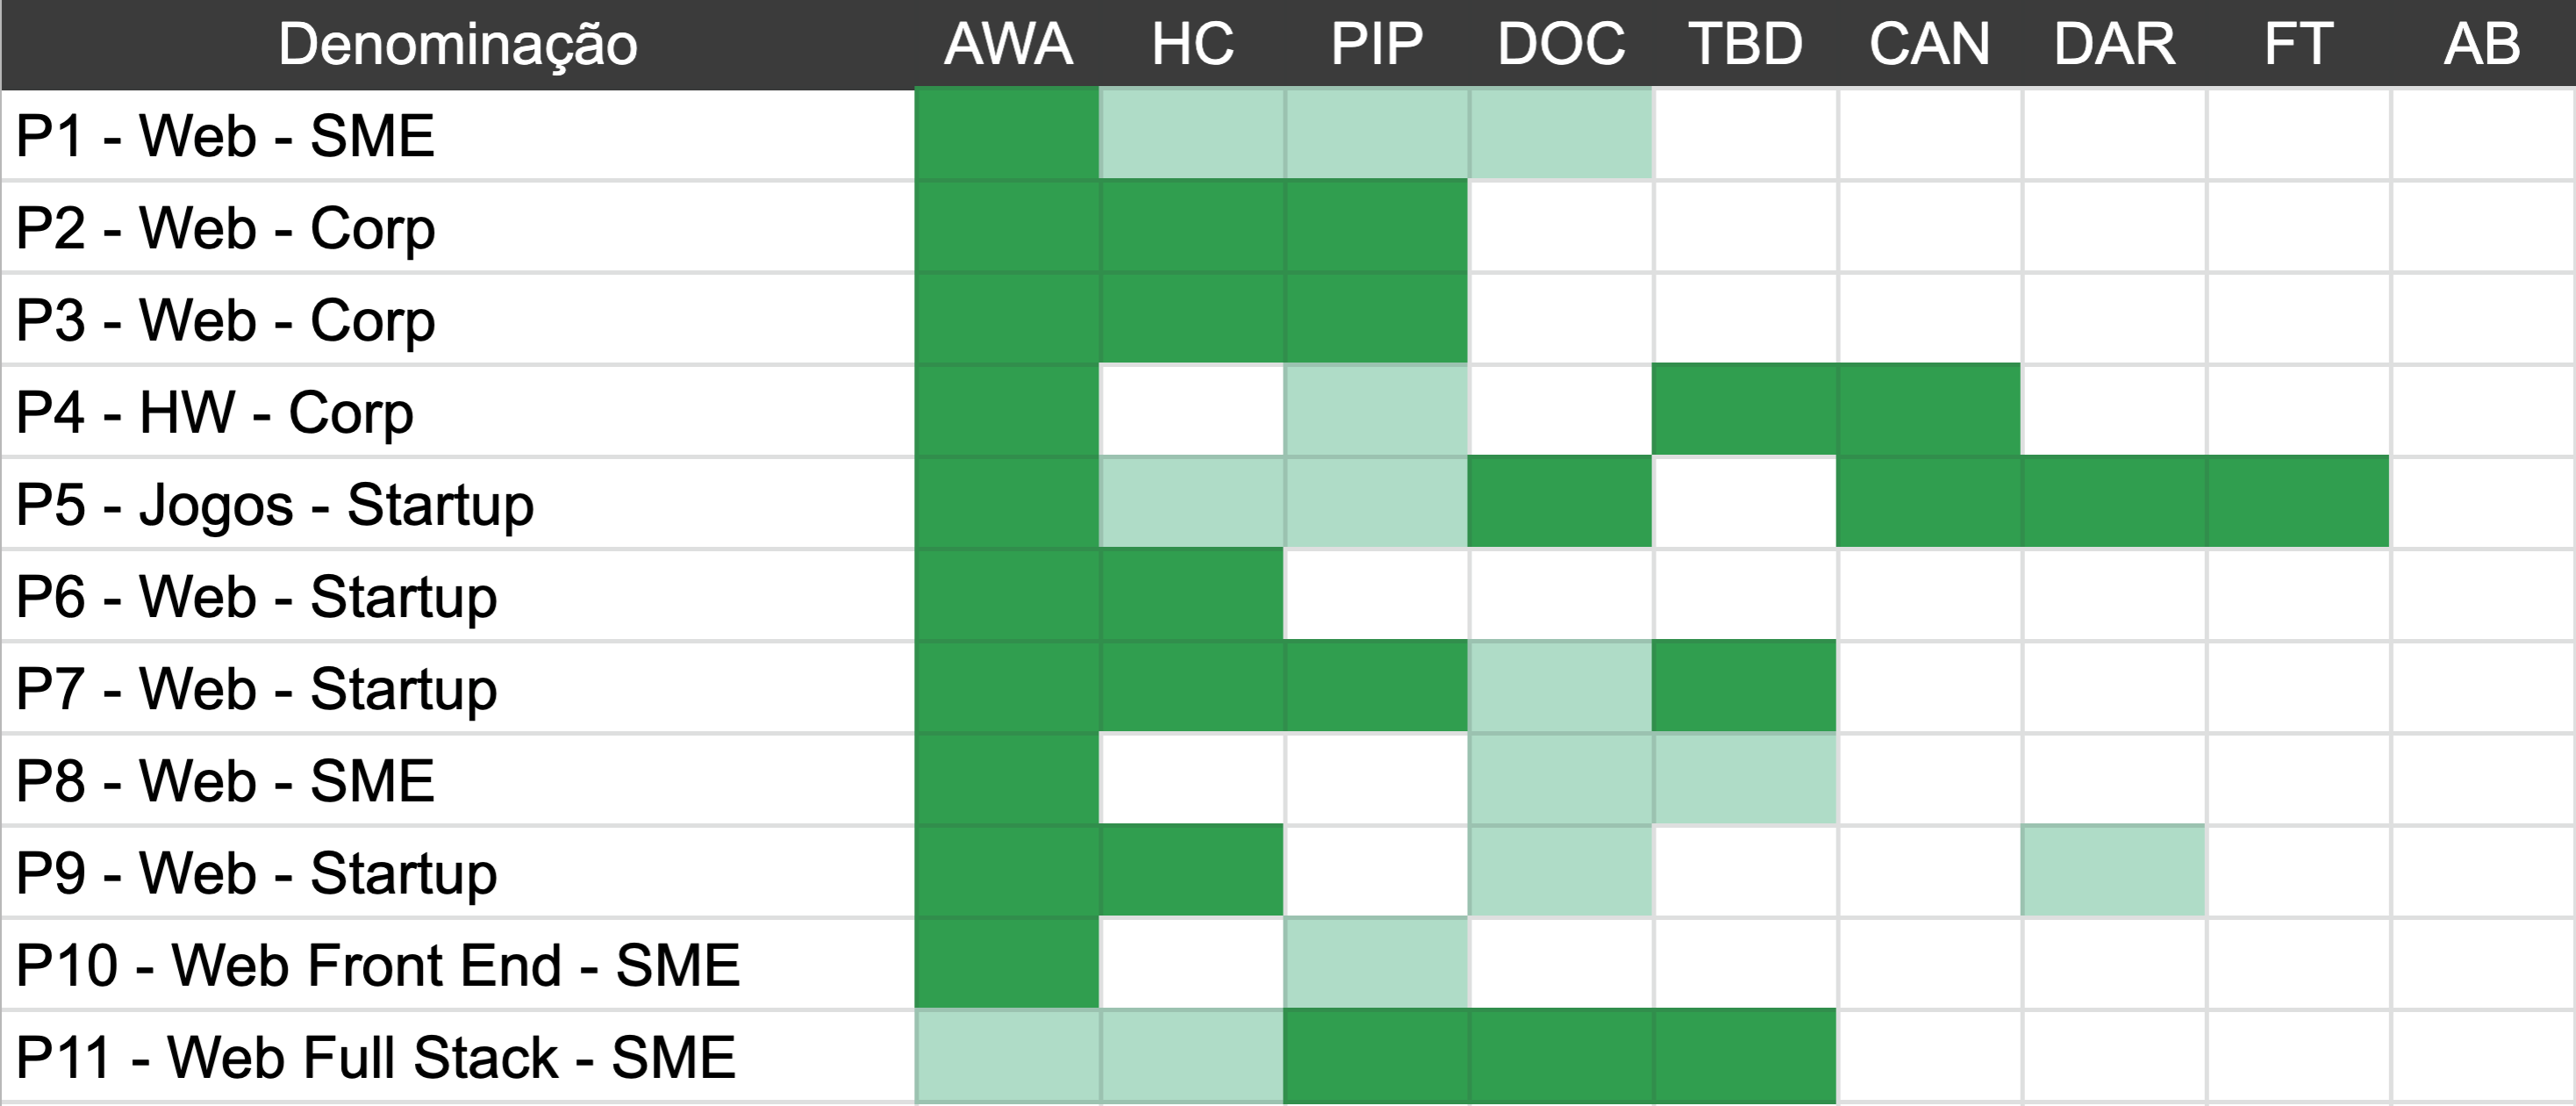
\includegraphics[width=\linewidth]{tabelaT3.png}
\end{center}
\caption[Nível de utilização das práticas, com as colunas em ordem decrescente de uso]{
    Nível de utilização de cada uma das práticas, com as colunas ordenadas em ordem decrescente de uso. Práticas: AWA: \emph{Developer Awareness}; HC: \emph{Health Check}; PIP: Pipeline de Implantação; DOC: \emph{Developer on Call}; TBD: \emph{Trunk Based Development}; CAN: \emph{Canary Releases}; DAR: \emph{Dark Launches}; FT: \emph{Feature Toggles}; AB: Testes A/B.
}\label{tabela_t3}
\end{table}

\begin{figure}[ht]
\begin{center}
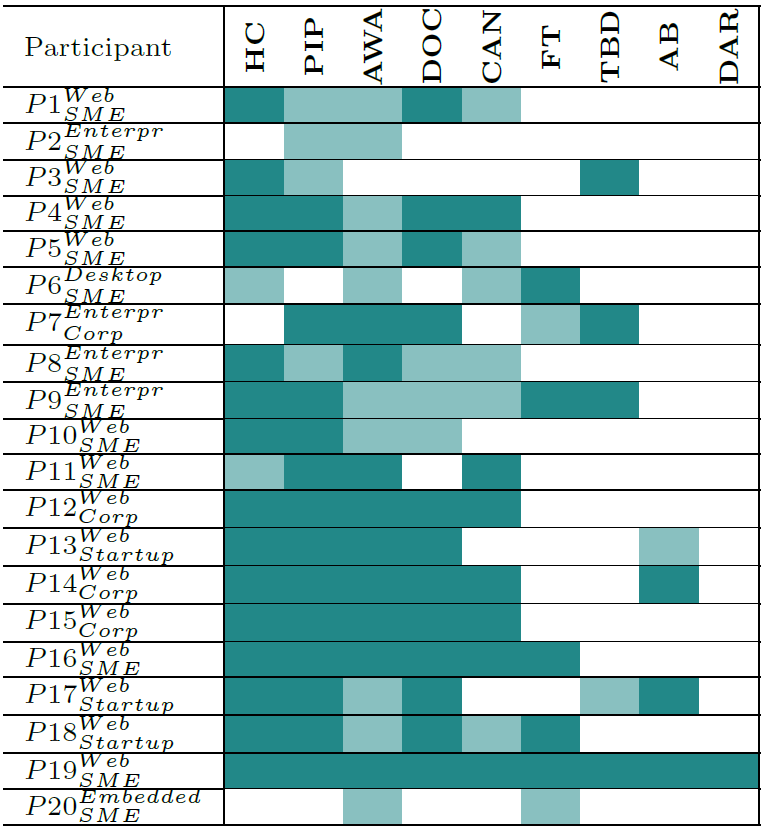
\includegraphics[width=\linewidth]{tabela1-artigo-base.png}
\end{center}
\caption[Tabela 1 do artigo base]{
    Utilização das práticas pelos participantes do artigo base.
    Fonte: Schermman et al \cite{empiricalStudy2016}. Práticas: AWA: \emph{Developer Awareness}; HC: \emph{Health Check}; PIP: Pipeline de Implantação; DOC: \emph{Developer on Call}; TBD: \emph{Trunk Based Development}; CAN: \emph{Canary Releases}; DAR: \emph{Dark Launches}; FT: \emph{Feature Toggles}; AB: Testes A/B.
}\label{tabela_1_artigo_base}
\end{figure}

Com a Tabela \ref{tabela_t3} é possível perceber que \emph{Developer awareness [AWA]} foi a prática mais encontrada em toda a amostra, sendo totalmente utilizada pela grande maioria dos entrevistados; apenas um deles utiliza parcialmente. Logo após, pode-se encontrar as práticas de \emph{Health Check} [HC] e Pipeline de Implantação [PIP]  na segunda e na terceira colocação, respectivamente. No geral, também pode-se inferir que as técnicas de \emph{Partial Rollouts} são ainda muito pouco utilizadas, com as 3 práticas do grupo entre as quatro últimas colocadas. Vale a pena citar que nenhum dos entrevistados utiliza, mesmo que precariamente, a técnica de Testes A/B [AB].

Quando comparamos a Tabela \ref{tabela_t3} com a Tabela 1 do artigo base (Figura \ref{tabela_1_artigo_base}), podemos perceber que há diferenças de posição entre práticas, mas que não há mudanças exorbitantes. Com a ajuda da Figura \ref{diferenca_entre_posicoes_fig}, é possível perceber que há uma diferença de no máximo 2 posições na ordem de predomínio, ao comparar os resultados obtidos neste trabalho com os do artigo base. É possível perceber que as práticas de AWA, TBD, DAR e FT tiveram mudanças de 2 posições, enquanto HC, PIP, CAN e AB tiveram apenas diferença de 1 unidade de posição. Apenas \emph{developer on call} permaneceu no mesmo local dentro das duas amostras. Por fim, é interessante perceber que o conjunto das três primeiras práticas é o mesmo, mas em posições trocadas nos dois estudos.

\begin{table}[ht]
\begin{center}
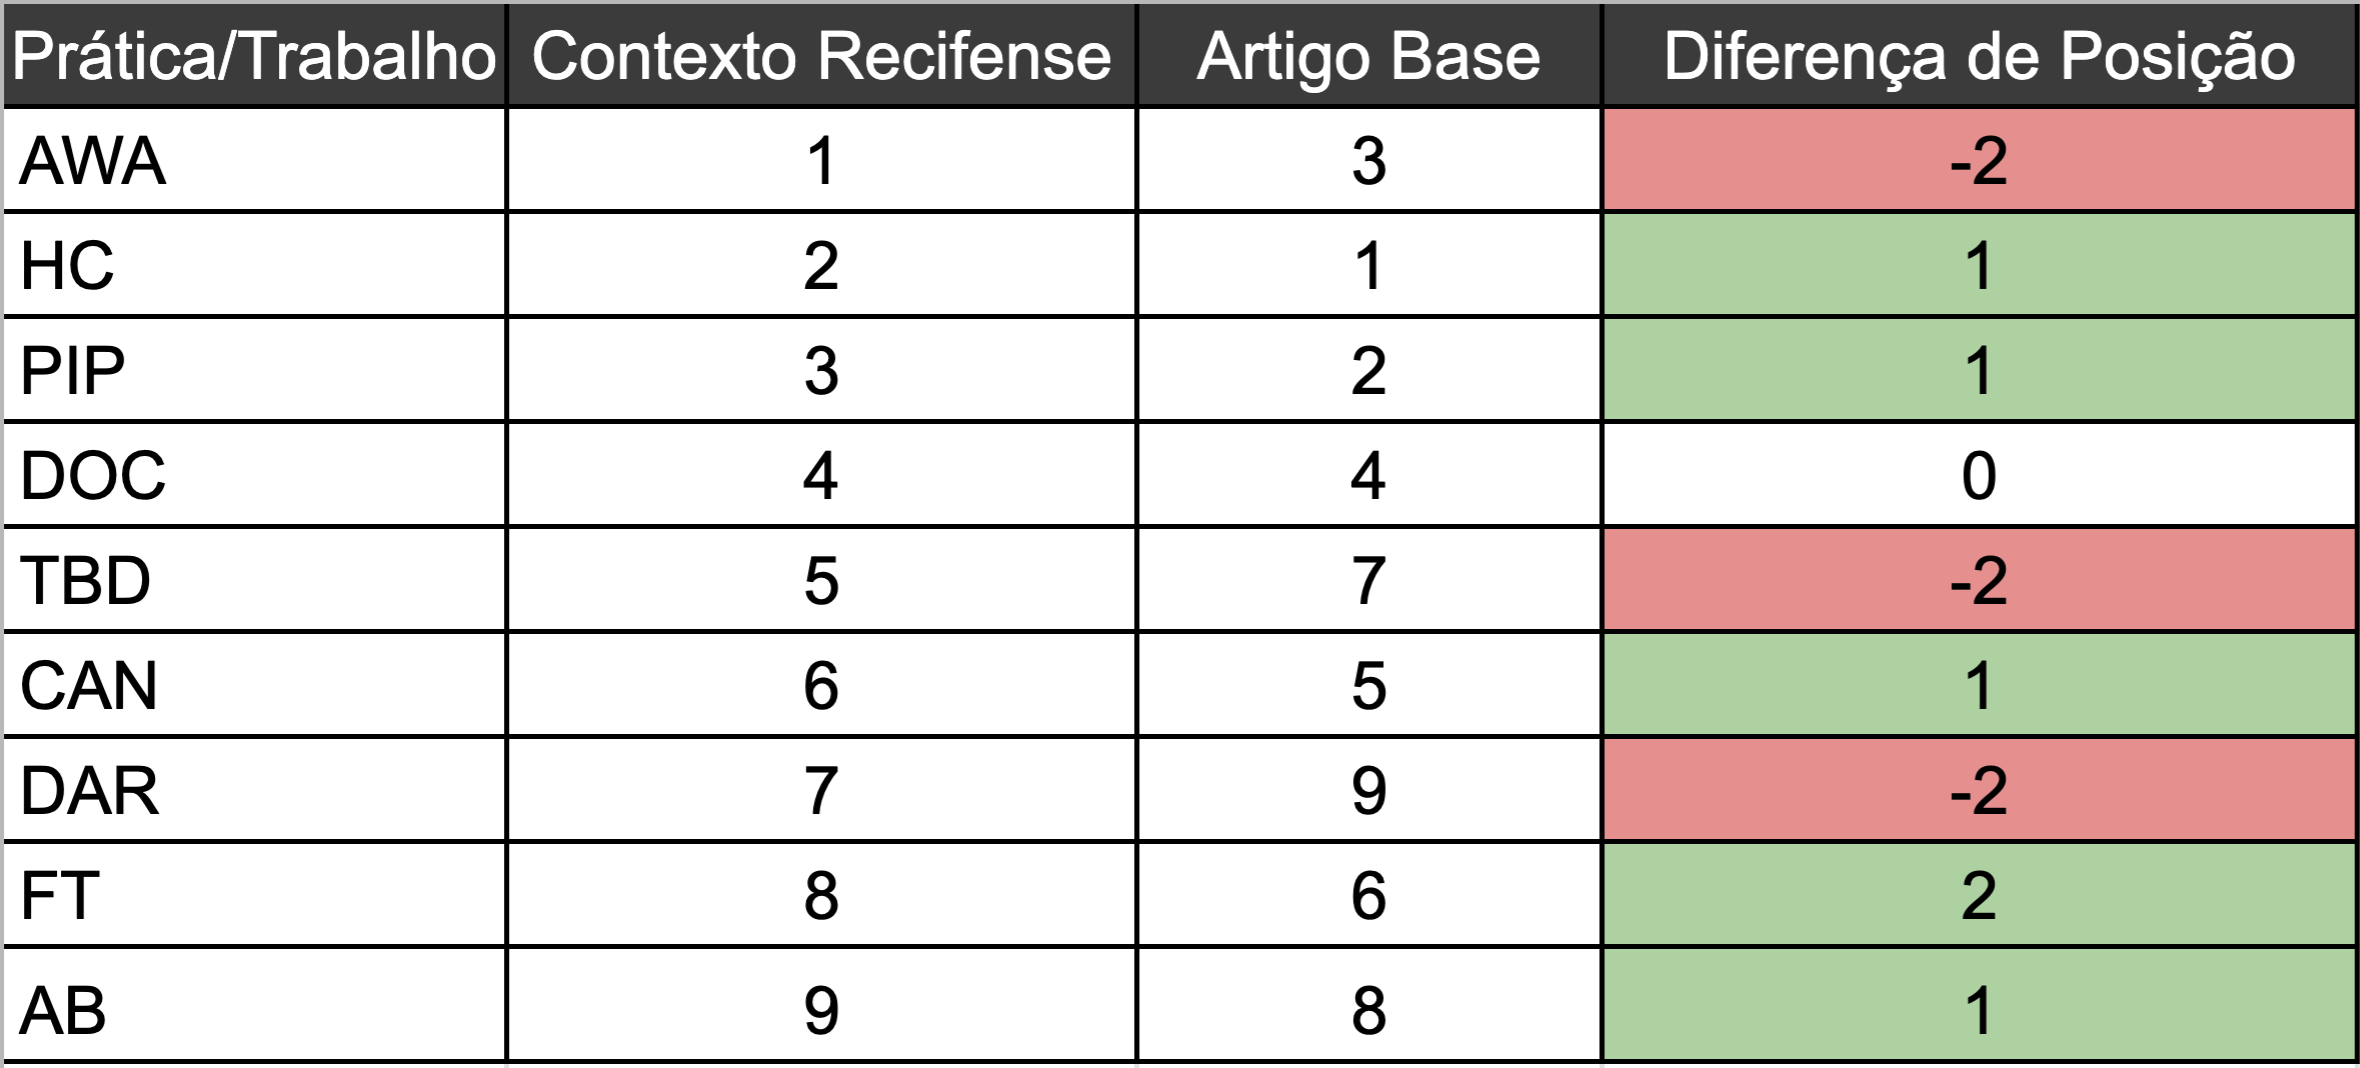
\includegraphics[width=\linewidth]{diferenca_entre_posicoes.png}
\end{center}
\caption[Diferença entre a ordem de predomínio das práticas]{
    Diferença entre o artigo base e este trabalho a respeito da ordem de predomínio das práticas. Práticas: AWA: \emph{Developer Awareness}; HC: \emph{Health Check}; PIP: Pipeline de Implantação; DOC: \emph{Developer on Call}; TBD: \emph{Trunk Based Development}; CAN: \emph{Canary Releases}; DAR: \emph{Dark Launches}; FT: \emph{Feature Toggles}; AB: Testes A/B.
}\label{diferenca_entre_posicoes_fig}
\end{table}

\subsection{Stairway to heaven}

Com o objetivo de responder a pergunta de pesquisa RQ2 -- \emph{O cenário de CI/CD nas empresas em Recife segue o ``stairway to heaven'' proposto no artigo?} -- foi produzida a Tabela \ref{tabela_t2}. Esta contém a visualização de utilização das práticas, utilizando a mesma técnica de cores aplicada na Tabela \ref{tabela_t3} e explicada na seção anterior, mas com as colunas ordenadas pela escada definida pela sequência de práticas do \emph{Stairway to Heaven} apresentada na Figura \ref{stairway} (Capítulo 3).

\begin{table}[ht]
\begin{center}
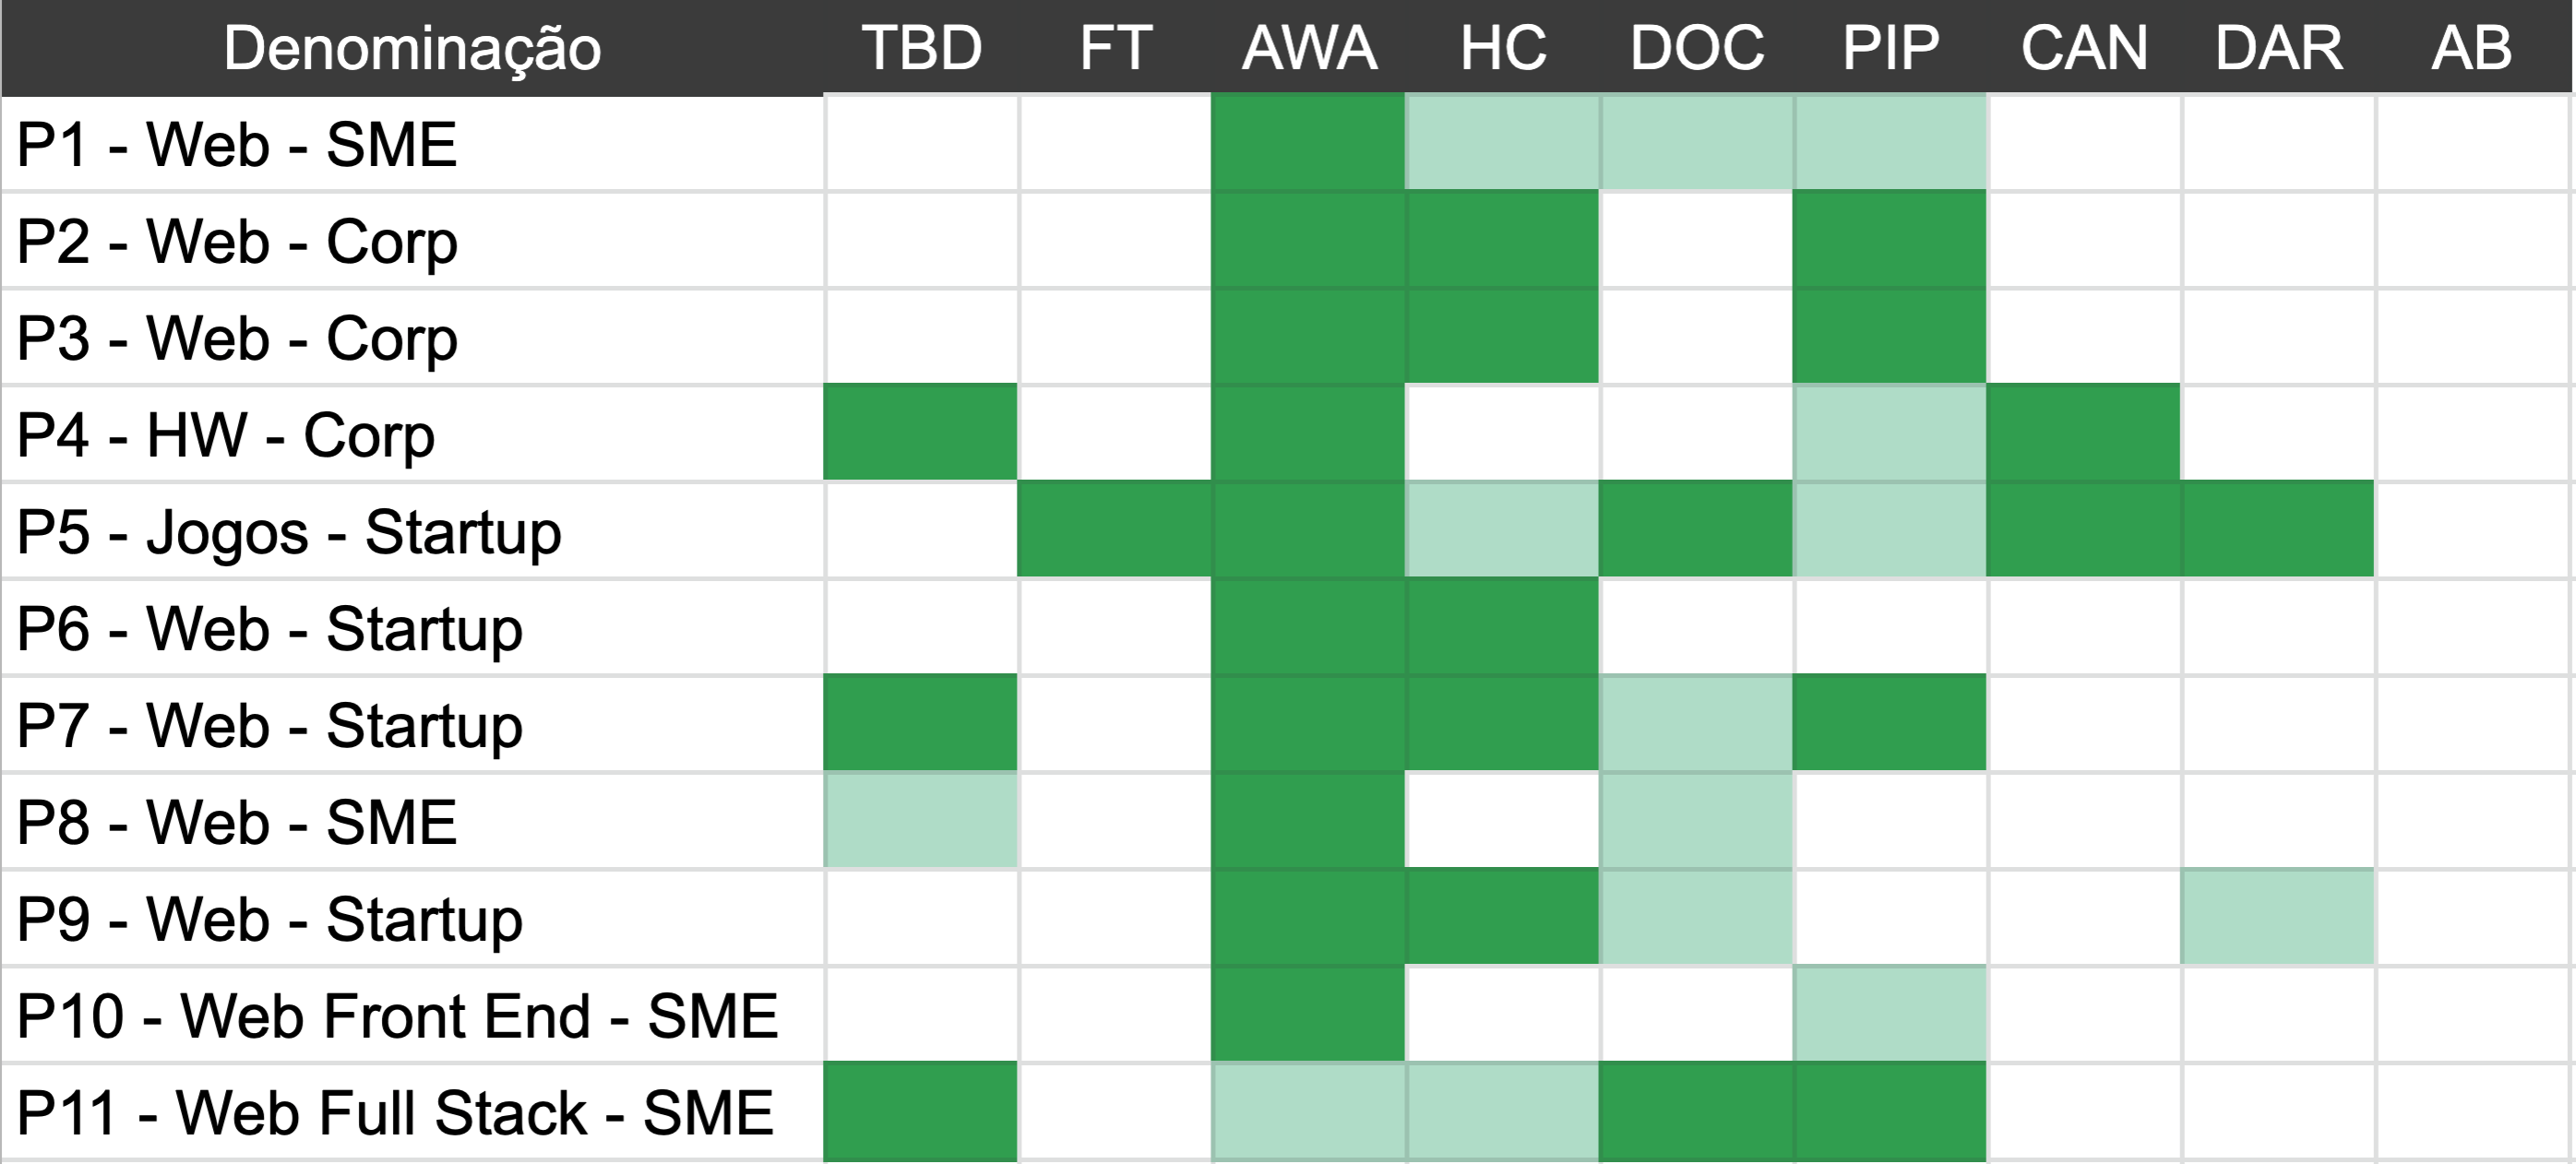
\includegraphics[width=\linewidth]{tabelaT2.png}
\end{center}
\caption[Nível de utilização das práticas, com as colunas na ordem do \emph{Stairway to Heaven}]{
    Nível de utilização de cada uma das práticas, com as colunas ordenadas na ordem do \emph{Stairway to Heaven}. Práticas: AWA: \emph{Developer Awareness}; HC: \emph{Health Check}; PIP: Pipeline de Implantação; DOC: \emph{Developer on Call}; TBD: \emph{Trunk Based Development}; CAN: \emph{Canary Releases}; DAR: \emph{Dark Launches}; FT: \emph{Feature Toggles}; AB: Testes A/B.
}\label{tabela_t2}
\end{table}

Com a Tabela \ref{tabela_t2} é possível perceber que a amostra deste estudo, assim como a amostra do estudo original, não segue a evolução proposta pelos autores do artigo base. Isso fica claro quando percebe-se que não há, em nenhum dos entrevistados, uma relação clara entre a coloração da coluna com a sua anterior. É possível notar também que há uma lacuna nas duas primeiras práticas, seguido de uma grande utilização da terceira, confirmando a tese de que a \emph{Stairway to Heaven} não foi identificada na amostra. O mais próximo dos participantes é P5, mas ainda há nele a falta do pilar TBD do primeiro degrau da escada. É interessante destacar que na amostra do próprio artigo base também não foi possível identificar a escada de evolução, como é possível visualizar na Figura \ref{tabela_1_artigo_base}.

\subsection{Análise das Práticas}

Nesta seção será abordado, para cada uma das práticas, as principais curiosidades encontradas na amostra. Esta tem como objetivo responder a pergunta RQ3: \emph{Quais são os princípios e práticas subjacentes que governam a adoção de CI/CD na indústria?} As seguintes subseções agrupam as práticas emergentes através das práticas gerais definidas no \emph{Stairway to Heaven}, inclusive seguindo a ordem deste, conforme explicado no Capítulo 4, Seção 4.4.

Para poder definir padrões encontrados na amostra, o autor, após a fase de agrupamento semântico, juntou todos os códigos e super categorias ligadas a cada uma das práticas, baseando-se principalmente na nota de utilização. Com a leitura e reflexão deste conjunto, o autor procurou por princípios que governam a adoção ou não de cada prática. Foi feito também um estudo comparativo com os resultados obtidos pelo artigo base para analisar discrepâncias e congruências entre os dois contextos de estudo.

\subsubsection{Integração Contínua}

Com a Tabela \ref{tabela_t3} é possível perceber que, apesar da grande disseminação a respeito de informações relacionadas a infraestrutura e manutenção de software -- ligadas à prática de \emph{Developer Awareness} \cite{awa} -- estar em primeiro lugar, as outras técnicas que compõem o conjunto de \emph{Continuous Integration} ainda não estão disseminadas na nossa amostra.

Nesta subseção, serão abordadas a seguir cada uma das práticas ligadas ao processo de Integração contínua, como explicado no Capítulo 2: \emph{Trunk Based Development} [TBD] \cite{devAndDeploymentFB}, \emph{Feature Toggles} [FT] \cite{featureToggles} e \emph{Developer Awareness} [AWA] .


\paragraph{Trunk Based Development [TBD]}
Na amostra é possível perceber que a técnica de \emph{Trunk Based Development} [TBD] não é tão amplamente adotada, visto que apenas 4 entrevistados utilizam ao menos parcialmente. Destes, 2 comentam que entregam novas versões aos clientes baseados em novas funcionalidades, e não em \emph{sprints}. Já entre os que não utilizam, 5 integram o código apenas no final da \emph{sprint}. Deste grupo, 2 utilizam a metodologia \emph{Git Flow} \cite{gitFlow}, que define uma maneira de manusear várias branches ao mesmo tempo de modo que os desenvolvedores deparem-se com o mínimo de conflitos possível e que software seja entregue em versões bem definidas.

\paragraph{Feature Toggles [FT]}

No estudo foi possível perceber que, na amostra, a prática de \emph{Feature Toggles} [FT] é raramente utilizada, assim como no artigo base. Esta técnica foi encontrada apenas na equipe do participante P5, que a utilizava para esconder funcionalidades enquanto testes manuais ainda estavam sendo feitos. Geralmente esta técnica é utilizada para auxiliar a integração de códigos ainda não finalizados quando a equipe utiliza técnicas como o \emph{trunk based development}, mas este não é o caso de P5. É interessante notar que este participante também foi um dos poucos que utilizava a técnica de \emph{Canary Releases} [CAN].

Entre o grupo dos que não utilizavam, 7 só enviam código novo para produção quando a funcionalidade está concluída. Deste grupo, 2 comentaram que fazem uso de conceito de épicos, onde uma história de usuário se prolonga por mais do que apenas uma sprint. É também interessante notar que P3 está em vias de utilizar esta técnica para reduzir conflitos de \emph{merge} e \emph{rebase} devido ao grande número de desenvolvedores em seu time, como podemos ver na citação:


\begin{quote}
    ``O meu time tem 23 [pessoas]. [...] a gente tá trabalhando em funcionalidades muito distintas, então às vezes acontece de termos um paralelismo de branches muito grande. [...] é muito complicado `mergear' e fazer \emph{rebase} de tudo. Realmente dá muitos conflito'' --- P3 -- Web -- CORP
\end{quote}


\paragraph{Developer Awareness [AWA]}

Na amostra é possível identificar que a prática de \emph{Developer Awareness} [AWA] é amplamente adotada nas companhias, assim como na amostra do artigo base. Em 6 entrevistas foi possível perceber que o time de desenvolvimento era o mesmo responsável pela entrega e manutenção da aplicação. Em outras 2, há um time específico de \emph{DevOps}, mas não havia grandes silos entre este e a equipe de desenvolvimento. Um caso interessante foi o de P11, que, apesar de um conhecimento espalhado dentro da equipe, há receio e insegurança por parte de alguns a respeito de questões de infraestrutura no geral.


\paragraph{Deployment Contínuo}

Nesta subseção, serão abordadas as práticas ligadas ao processo de \emph{Deployment} contínuo, como explicado no Capítulo 2: \emph{Health Checks} [HC] \cite{devopsBook}, \emph{Developer on Call} [DOC] \cite{devAndDeploymentFB} e Pipeline de Implantação [PIP] \cite{devopsBook}. É possível inferir, baseado principalmente na Tabela \ref{tabela_t3}, que as técnicas ligadas ao processo estão presentes na maioria das equipes da amostra: as 3 estão nas quatro primeiras colocações. 

\paragraph{Health Checks [HC]}

Sobre a prática de \emph{Health Checks} [HC], é possível perceber que, apesar de não ser o mais adotado -- como foi no artigo base, ainda tem destaque entre as outras, presente na segunda colocação. Na amostra, 7 entrevistados continham pelo menos uma forma rudimentar de verificação e alertas, e destes, 2 continham apenas verificações não muito complexas. Um ponto interessante que surgiu foi o fato de P4 achar que não era necessário utilizar esta técnica por estar em fase de prototipação.

\paragraph{Developer on Call [DOC]}

Na amostra é possível perceber que a técnica de \emph{Developer on Call} [DOC] é mais adotada de forma implícita do que de fato definida -- 3 entrevistados estão em times que funcionam desta forma. Contudo, 5 pessoas do grupo não utilizam esta prática: alguns comentaram que a confiança nos testes automáticos faz com que não utilizem a prática, enquanto outro comentou que a prática é inclusive mal vista pela empresa.

Uma dicotomia interessante foi encontrada entre os resultados da amostra deste trabalho e o do artigo base. Este último comenta que a prática já está sendo largamente aceita nas organizações atualmente, e inclusive um dos entrevistados comenta que essa responsabilidade de ficar até mais tarde para resolver problemas leva os desenvolvedores a escreverem e testarem seus códigos mais veementemente. Tal argumentação tem como base a seguinte citação retirada do artigo e traduzida:

\begin{quote}
    ``Se você não tem testes suficientes e faz deploy de um código ruim isso vai se voltar contra você pois você estará de plantão e terá que dar suporte a isto.'' --- P14 (do artigo base) -- Web -- CORP
\end{quote}


Contudo, com a seguinte citação de P2, é possível perceber que há um sentimento contrário: confia-se no processo de qualidade e, por isso, não necessitam de plantão.


\begin{quote}
    ``Temos o ciclo de QA, se encontrar alguma coisa a gente vê […] não precisa isso de plantão não.'' --- P2 -- Web -- CORP
\end{quote}

\paragraph{Pipeline de Implantação [PIP]}

Em relação à prática de Pipeline de Implantação [PIP] é possível inferir que ela é amplamente adotada pela amostra, visto que apenas 2 entrevistados obtiveram nota 0 (não utiliza). No artigo base é possível perceber um resultado semelhante a este. Uma grande parte dos entrevistados segue o mesmo padrão para qualquer tamanho da mudança. Outros 2 tinham alguns processos automatizados, mas a \emph{pipeline} era diferente dependendo do tamanho da mudança.

É interessante perceber que alguns times ainda demonstram falta de automação dos processos da \emph{pipeline}. Isto acontece em decorrência da complexidade da automação, devido às tecnologias e ferramentas utilizadas, ou da falta de prioridade do time para tal.
 
\paragraph{Entregas Parciais}

Nesta subseção, serão abordadas as práticas ligadas ao processo de Entregas Parciais, como explicado no Capítulo 2: \emph{Canary Releases} [CAN] \cite{continuousDeliveryBook}, \emph{Dark Launches} [DAR] \cite{devAndDeploymentFB} e Testes A/B [AB] \cite{testsAB}. Na amostra foi possível perceber que todas as técnicas são muito pouco utilizadas: todas estão entre as 4 últimas colocações. É válido também notar que as 3 mantiveram a mesma ordem de utilização do processo do artigo base \cite{empiricalStudy2016}.

\paragraph{Canary Releases [CAN]}

A técnica de \emph{Canary Releases} [CAN] apareceu nos contextos de jogos e no de sistemas embarcados. Na equipe do entrevistado P5, que trabalha no domínio de jogos eletrônicos, os principais jogadores -- conhecidos como ``baleias'' -- são escolhidos para participar de um \emph{early access} de novas funcionalidades.  Esses testes levam em torno de 1 semana. 

Já na equipe de P4, que trabalha com sistemas embarcados, a prática era necessária devido ao contexto de atuação e às tecnologias utilizadas. Como o sistema que está em fase de prototipação servirá para o contexto médico, vários testes de campo deveriam ser feitos para garantir que todas as funcionalidades estivessem de acordo com o esperado. Para os testes, o cliente que contratou a empresa de P4 escolhia a quantidade de pessoas e local que serviria como validação de funcionalidades.

Entre os entrevistados que não utilizam a prática de \emph{Canary Releases}, 3 têm um ambiente de homologação para testes e validação de requisitos, mas este utiliza dados diferentes dos de produção. Outros 3 comentam que as features são sempre entregues para todos os usuários ao mesmo tempo.


\paragraph{Dark Launches [DAR]}

Do grupo das práticas associadas a Entregas Parciais, \emph{Dark Launches} [DAR] foi a segunda mais utilizada, mas a menos conhecida entre os entrevistados. Isto se confirma com o fato de que 6 entrevistados disseram nunca ter utilizado, e 3 destes disseram especificamente que não conheciam a técnica. Importante notar que no estudo base \cite{empiricalStudy2016} esta é a menos utilizada do grupo de práticas.

\emph{Dark Launches} foi utilizado totalmente por P5 no contexto de jogos para testes manuais, e apenas parcialmente no contexto de WEB por P9 para validações de alguns cenários que dependiam de dados de produção.


\begin{quote}
    ``A gente implementa a funcionalidade mas condiciona a não aparecer para o usuário até que a gente queira.'' --- P5 -- Jogos -- Startup
\end{quote}

\paragraph{Testes A/B [AB]}

A prática de Testes A/B [AB] não foi identificada em nenhum dos participantes. Entre as principais causas levantadas para tal, 4 entrevistados comentaram que não utilizam pela baixa quantidade de usuários ativos no sistema. Outros 2 comentaram que a técnica não se aplicava ao contexto da aplicação. É interessante notar que esses dois motivos estão presentes no artigo base \cite{empiricalStudy2016}, contudo, ao contrário deste, ninguém na amostra comentou sobre problemas na arquitetura como causa para não utilização.


\begin{quote}
    ``O sistema da gente -- apesar de lidar com uma massa de dados muito grande -- não têm tantos usuários, então não faz muito sentido [utilizar testes A/B]....'' --- P2 -- WEB -- Corp
\end{quote}

Outro motivo importante foi levantado por P8, que comenta que aparentemente não existe na empresa o interesse em investir nessa prática. P3 comenta ainda que o time está mais focado em entregar novas funcionalidades, pois a demanda por parte do cliente é muito grande.

\subsection{Descobertas adicionais}

Esta subseção abordará sobre os dois tópicos marginais que foram levantados durante a análise dos dados obtidos pelas entrevistas: \emph{Code Review} e testes automáticos.

\paragraph{Code Review}

A prática de \emph{Code Review} \cite{codeReview} é bem vista pela maioria dos entrevistados, considerado uma técnica importante e essencial para o controle de qualidade de código. As razões para o uso são diversas, desde de impor boas práticas -- por P7 -- até o compartilhamento e nivelamento do conhecimento -- por P11.

\begin{quote}
    ``... a partir do momento que o sistema vai crescendo, o próprio desenvolvedor não tem a noção de que aquela sua mudança não é a melhor forma de fazer e que pode quebrar outras partes do sistema...'' --- P2 -- WEB -- Corp
\end{quote}

Ainda na amostra, 3 entrevistados acreditam que a prática funciona principalmente para troca de conhecimento. Sobre isso, a entrevistada P10 comenta que agrega muito valor para ela como novata no time, mas acha que adiciona um tempo desnecessário na entrega de funcionalidades por pessoas mais experientes, visto que -- para ela -- a técnica não faria sentido neste caso.

Outro ponto importante foi a distinção entre dois relatos a respeito do engajamento do time com a prática. Enquanto P3 comenta que a equipe dela é bem aberta ao debate e está engajada com o processo, P7 fala que o processo funciona ``mais ou menos'', dependendo do humor dos revisores.

\paragraph{Testes Automáticos}

Testes automáticos são, no geral, bem vistos e extremamente recomendados pela maioria dos entrevistados como forma de prevenir erros em tempo de execução. Contudo, o participante P2 comenta que ainda é contrário a depender somente deles como garantia de qualidade.

\begin{quote}
    ``... automação [de testes] não resolve todos os problemas [relacionados a garantia de qualidade], ele vai identificar muita coisa, mas tem várias outras que precisamos do olhar de um testador…'' --- P2 -- WEB -- Corp
\end{quote}

Na amostra, 5 entrevistados acreditam que o aumento da cobertura de testes automáticos pode diminuir a quantidade de bugs em produção. Dentro desse grupo, o participante P9 comenta que isto poderia, no entanto, diminuir a velocidade de entregas do time. P5 adicionou ainda que sente que a \emph{sprint} é muito curta e não consegue tempo dentro destas para adicionar testes automáticos.

\subsection{Ameaças a validade}

Mesmo com a metodologia definida e seguida utilizando métodos conhecidos pela comunidade científica, é necessário levantar possíveis ameaças à validade dos resultados encontrados neste trabalho. Uma ameaça plausível é a quantidade relativamente pequena de entrevistas feitas.

É importante salientar também que os códigos gerados durante o processo de codificação das entrevistas sofreram um certo enviesamento visto que este trabalho é uma replicação de um estudo, então o autor tinha em mente que assuntos estavam sendo procurados na fala durante o levantamento de códigos. 

Outra ameaça que deve ser levada em conta é o processo de \emph{coding} realizado. Ele foi feito baseando-se no áudio das entrevistas, e não nos textos transcritos, como geralmente é feito \cite{groundedTheory}. Isso pode tornar os códigos enviesados ou até mesmo significar a falta de códigos importantes que poderiam ter sido levantados pelo processo original. É válido citar que há algumas vertentes que defendem a codificação através do áudio, por preservar a entonação e a intenção do usuário, mas ainda devem ser feitos trabalhos quantitativos na área para validação e melhor definição do processo \cite{listenCode}. 
